\documentclass[12pt]{article}

%Filter Warning messages, otherwise it would stuff like 
\usepackage{silence}
%Disable all warnings issued by latex starting with "You have..."
\WarningFilter{latex}{You have requested package}

%Allgemeine Einstellungen

%Abstände
\usepackage[a4paper,left=3cm,right=3cm,top=2.5cm,bottom=3.5cm,headsep=12pt]{geometry}%Bottom extra 0.5cm für Footer

%Deutsches Sprachpacket
\usepackage[german,ngerman]{babel}

%Times New Roman
\usepackage{mathptmx}

%Titelseite einbinden
\usepackage{pdfpages}

%1.5-Zeilenabstand
\usepackage[onehalfspacing]{setspace}

%Stil der Überschriften, siehe ueberschriften.sty
\usepackage[numeric]{../../ueberschriften}

%Stil des Inhaltsverzeichnisses, siehe inhaltsverzeichnis.sty
\usepackage[numeric]{../../inhaltsverzeichnis}

%Abkürzungsverzeichnis, siehe abk_verzeichnis.sty
\usepackage{../../abk_verzeichnis}

%Stil der Fußzeilen, siehe fusszeilen.sty
\usepackage{../../fusszeilen}

%Literaturverzeichnis und Zitate, siehe literatur.sty
\usepackage{../../literatur}

%Stil für Header und Footer, siehe header_footer.sty
%Wenn nicht erwünscht, müssen auch die Befehle \frontmatter, \mainmatter auskommentiert werden
\usepackage{../../header_footer}

%Stile für Code-Ausschnitte, siehe codes.sty
\usepackage{../../codes}

%Stile für Anhänge, Bilder, ...
\usepackage{../../anhang}

%Silbentrennung (manche Worte werden am Zeilenende nicht getrennt, diese müssen dann nachgetragen werden)
\usepackage[T1]{fontenc}
\hyphenation{öf-fent-lich-en}

%DEBUGGING (Zeigt Boxen an)
%\usepackage{showframe}
\setlength{\skip\footins}{12pt}

\usepackage{makecell}
\usepackage{placeins}

\fancypagestyle{main}{%
  \fancyhf{}%
  \fancyhead[L]{}%
  \fancyhead[R]{\nouppercase\parttitle}%
  \fancyfoot[L]{\myauthor}%
  \fancyfoot[R]{\thepage}%
  \renewcommand{\headrulewidth}{0.4pt}%
  \renewcommand{\footrulewidth}{0.4pt}%
}

\fancypagestyle{plain}{%
  \fancyhf{}%
  \fancyhead[L]{}%
  \fancyhead[R]{\nouppercase\plaintitle}%
  \fancyfoot[L]{\myauthor}%
  \fancyfoot[R]{\thepage}%
  \renewcommand{\headrulewidth}{0.4pt}%
  \renewcommand{\footrulewidth}{0.4pt}%
}

\useInlineCites

%\setlength{\skip\footins}{6pt}

\begin{document}

\renewcommand{\mytitle}{Entwicklung und Bewertung eines Kennzahlen-\\systems für nachhaltige Kryptowährungen}%Titel für oben links
\renewcommand{\myauthor}{Michael Eing, Vanessa Kriebel,\\Timo Stovermann, Bastian Wynk}%Name für unten links
\renewcommand{\headheight}{27pt}%Bei Mehrzeiligem Titel muss Headerhöhe angepasst werden


\includepdf[pages={1-}]{titelseite.pdf}

\frontmatter%Stil des Headers/Footers ändern

\pagenumbering{Roman}

\addcontentsline{toc}{part}{Abkürzungsverzeichnis}%Abk-Verz. ins Inhaltsverzeichnis
\printabbreviations%abk_verzeichnis.sty
\clearpage
\renewcommand{\plaintitle}{Abbildungsverzeichnis}
\addcontentsline{toc}{part}{Abbildungsverzeichnis}
{\def\makebox[#1][#2]#3{#3}%
\listoffigures
}
\clearpage
\renewcommand{\plaintitle}{Inhaltsverzeichnis}%Titel für oben Rechts
%Defbox, damit gepunktete Linie bis zur Zahl geht
{\def\makebox[#1][#2]#3{#3}%
	\tableofcontents
}

\addtocontents{toc}{\vspace{24pt}}%Freiraum im ToC

\clearpage
\mainmatter%Stil des Headers/Footers ändern
\pagenumbering{arabic}

\part{Einleitung}
Mit der Einführung des Internets ist es möglich geworden, auf einfachem Wege weltweit mit anderen Menschen zu kommunizieren und Informationen auszutauschen. Diese Gegebenheit ist unter anderem dazu genutzt worden, eine globale Handelsplattform unter den Nutzern zu schaffen. So haben sich mit der Zeit verschiedenste Onlineshops gebildet, die es ermöglichen, Güter und Waren aus der ganzen Welt zu erwerben. Ein Hindernis für diese globale Handelsmethode stellen jedoch die weltweit unterschiedlichen Währungen dar, da diese keinen einheitlichen Zahlungsverkehr ermöglichen. Im Jahre 2009 kam es zu einer ersten Idee, dieses Problem mittels einer einheitlichen Währung zu lösen. Mit der Einführung des Bitcoins, der ersten Kryptowährung, wurde ein globales, dezentrales Zahlungsmittel geschaffen, welches ausschließlich im Internet gehandelt werden konnte und keinen physikalischen Wert in der realen Welt wie herkömmliches Geld besitzt\citebib{neumann}{S.2}{vgl. }. Die Schaffung des Bitcoins hatte mit ihrer Idee einer Kryptowährung die Geburt vieler weiterer Kryptowährungen zur Folge. In den folgenden Unterkapiteln wird nun grob darauf eingegangen, welche Eigenschaften diese Kryptowährungen haben und wie das Ganze technologisch (am Beispiel Bitcoin) in der Praxis umgesetzt wird.

\part{Einführung in Kryptowährungen}
Mit der Einführung des Internets ist es möglich geworden, auf einfachem Wege weltweit mit anderen Menschen zu kommunizieren und Informationen auszutauschen. Diese Gegebenheit ist unter anderem dazu genutzt worden, eine globale Handelsplattform unter den Nutzern zu schaffen. So haben sich mit der Zeit verschiedenste Onlineshops gebildet, die es ermöglichen, Güter und Waren aus der ganzen Welt zu erwerben. Ein Hindernis für diese globale Handelsmethode stellen jedoch die weltweit unterschiedlichen Währungen dar, da diese keinen einheitlichen Zahlungsverkehr ermöglichen. Im Jahre 2009 kam es zu einer ersten Idee, dieses Problem mittels einer einheitlichen Währung zu lösen. Mit der Einführung des Bitcoins, der ersten Kryptowährung, wurde ein globales, dezentrales Zahlungsmittel geschaffen, welches ausschließlich im Internet gehandelt werden konnte und keinen physikalischen Wert in der realen Welt wie herkömmliches Geld besitzt\citebib{neumann}{S.2}{vgl. }. Die Schaffung des Bitcoins hatte mit ihrer Idee einer Kryptowährung die Geburt vieler weiterer Kryptowährungen zur Folge. In den folgenden Unterkapiteln wird nun grob darauf eingegangen, welche Eigenschaften diese Kryptowährungen haben und wie das Ganze technologisch (am Beispiel Bitcoin) in der Praxis umgesetzt wird.

\section{Dezentralisierung}
Der erste wichtige Baustein und eine der bedeutendsten Eigenschaften von Kryptowährungen ist die Dezentralisierung. Das bedeutet, dass weder der Handel, noch die Ausgabe von Kryptowährungen zentral von einem Staat oder von einer Bank abgewickelt werden, was bei herkömmlichen Währungen hingegen der Fall ist. Die Ausgabe und der Handel finden ausschließlich im Internet unter den Nutzern direkt statt und dies sorgt so für eine Unabhängigkeit von übergeordneten Instanzen, welche sich sonst um die Verwaltung kümmern müssten\citebib{neumann}{S.4}{vgl. }.\\
Die technische Grundlage hierfür bildet ein Peer-to-Peer Netzwerk (P2P). Peer-to-Peer Netzwerke sind Rechnernetze, bei denen alle Rechner im Netz miteinander verbunden sind und gleichberechtigt miteinander arbeiten\citebib{hoenig}{S.35}{vgl. }. Jeder Rechner kann Funktionen und Dienstleistungen anbieten und von anderen Rechnern angebotene Funktionen, Ressourcen, Dienstleistungen und Dateien nutzen. Zudem kann jeder Rechner mit mehreren anderen Rechnern verbunden sein. Die Daten sind dabei in der Regel auf den Rechnern der Nutzer verteilt. Es handelt sich hier demzufolge um ein dezentrales Konzept, da es keinen übergeordneten, zentralen Server zur Verwaltung gibt\citebib{neumann}{S.6}{vgl. }.\\
Das Peer-to-Peer Netzwerk von Kryptowährungen basiert auf einer von allen Nutzern gemeinsam genutzten und verwalteten (also dezentralen) Datenbank, in der alle Transaktionen zwischen den Nutzern überwiegend in einer sogenannten Blockchain gespeichert werden. Diese Art der Datenverwaltung wird auch Distributed-Ledger-Technologie, kurz Ledger genannt. Das Netzwerk bzw. der Ledger fungiert dabei wie ein globales, kollektives Buchführungssystem mit dem Zweck, das Verdoppeln oder Fälschen der Kryptowährung zu verhindern\citebib{neumann}{S.7}{vgl. }.\\
Im Gegensatz zu einem klassischen Kassenbuch, wo die Daten auf einem einzigen System gespeichert und von einer zentralen Instanz gepflegt werden, sind die Informationen bei einer Blockchain auf eine große Anzahl von Netzwerkteilnehmern, sogenannte „Knoten“, verteilt. Die Knoten vertrauen sich gegenseitig nicht und das Kassenbuch wird mehrfach abgespeichert. Das hat zur Folge, dass eine Vielzahl von Computern weltweit identische Kopien der gesamten Transaktionshistorie besitzen. Diese dezentrale Art der Datenorganisation hilft dabei, Angriffe auf das Netzwerk zu verhindern und das Vertrauen in die erfassten Daten zu erhöhen\citebib{schuster}{S.4}{vgl. }.

\section{Wallets und die digitale Signatur}
Zur Verwendung der digitalen Währung besitzt jeder Nutzer eine sogenannte Wallet (Portemonnaie), wodurch es ihm möglich ist, sein Konto zu verwalten. Die hierfür nötige Clientsoftware wird durch verschiedene Anbieter im Internet vertrieben. Anders als bei einer herkömmlichen Wallet wird hier jedoch nicht direkt das Geld aufbewahrt. Stattdessen befinden sich hier die beiden Schlüssel zur eigenen Bitcoin-Adresse. So gibt es für jeden Benutzer ein Schlüsselpaar aus privatem und öffentlichem Schlüssel, welche beide zusammenpassen. Mit dem öffentlichen Schlüssel wird die eigene Bitcoin-Adresse für alle Clients im Netzwerk sichtbar\citebib{neumann}{S.7}{vgl. }. Durch den privaten Schlüssel wiederum kann der Absender seine Transaktion verschlüsseln – man spricht hier auch von „signieren“. Jeder beliebige Netzwerkteilnehmer kann nun die verschlüsselte Transaktion verifizieren, indem er diese mit dem öffentlichen Schlüssel entschlüsselt und so sicherstellen kann, dass sie tatsächlich vom Absender stammt. Auf diese Weise werden Authentizität und Integrität der einzelnen Transaktionen gewährleistet, denn man kann eine Transaktion ihrem Absendern zuordnen und gleichzeitig sicherstellen, dass sie nicht manipuliert wurden\citebib{schuster}{S.5f.}{vgl. }.\\
Wenn ein Nutzer eine Transaktion ausführen möchte, muss er mithilfe seines privaten Schlüssels seine Nachricht signieren. Die Nachricht wiederum beinhaltet dann die Informationen wie den Sender, den Empfänger und die Höhe des zu versendenden Betrags. Sobald die Nachricht ordnungsgemäß mit dem privaten Schlüssel signiert wurde, wird die Information des Versendens der Transaktion an alle Nutzer geschickt. Wenn eine gewisse Zeit vergangen ist (bei Bitcoin beispielsweise ungefähr 10 Minuten), werden die getätigten Transaktionen in einem Block zusammengefasst, von den Minern verifiziert und anschließend dem öffentlichen Transaktionsprotokoll, der sogenannten Blockchain, hinzugefügt\citebib{neumann}{S.11f.}{vgl. }. Miner könnte man als die „Verwalter“ des Systems bezeichne. Es handelt sich hier um eine Gruppe von Menschen, die großes Interesse an der korrekten Funktionsweise der Kryptowährung hat, aber in der Regel nicht in Kontakt zueinander stehen.

\section{Die Blockchain und Hash-Funktionen}
Alle getätigten Transaktionen innerhalb eines Netzwerks für Kryptowährungen werden aufgezeichnet und in einer Blockchain gespeichert. Es handelt sich hierbei um eine verteilte Open-Source-Datenbank, welche auf moderner Kryptografie basiert. Die Blockchain übernimmt zwei zentrale Aufgaben: sie bietet eine Methode zum Organisieren und Speichern von Daten und gleichzeitig eine Methode, um das Vertrauen in die Daten zu fördern\citebib{schuster}{S.3f.}{vgl. }.\\
Bei einer Blockchain werden die Informationen in einer stetig wachsenden Liste von Datensätzen organisiert. Wichtig ist hier, dass lediglich Daten hinzugefügt, aber frühere Daten nicht verändert oder gelöscht werden können. Bei Änderungen werden alte Einträge also nicht überschrieben, sondern neue Einträge erzeugt. Auch wenn diese Methode vergleichsweise umständlich und speicherintensiv ist, wird durch die Dokumentation der gesamten Historie die Transparenz und Betrugssicherheit stark gefördert. Die Transaktionsdaten werden dabei aus Effizienzgründen in Blöcken zusammengefasst\citebib{schuster}{S.4}{vgl. }.\\
Die Blockchain selbst besteht aus einer Aneinanderreihung dieser Blöcke (daher der Name „Blockchain“), wobei jeder Block die Transaktionsdaten von einem bestimmten Zeitraum beinhaltet. Dadurch fungiert die Blockchain als eine Art globales Kontobuch für das System. Ein sogenannter Miner hat dabei die Aufgabe, die Transaktionen eines Blocks zu bestätigen, damit man diesen wiederum zu der bestehenden Kette hinzufügen kann. Für das Erledigen der Aufgabe erhält der Miner eine Belohnung in Form der Währung des Systems\citebib{neumann}{S.8}{vgl. }.\\
Ein Block einer Blockchain besteht dabei aus drei Dingen: den Daten (im Fall von Kryptowährung den Transaktionsdaten), seinem eindeutigen Hash-Wert und dem Hash-Wert des vorherigen Blocks. Hash-Werte sind eine Aneinanderreihung von Zahlen und Buchstaben und werden mithilfe von Hash-Funktionen gebildet. Diese Hash-Funktionen sorgen dafür, dass eine große Datenmenge (wie zum Beispiel der gesamte Inhalt eines Blocks) auf eine kleine Datenmenge (den Hash-Wert) festgelegter Größe (beispielsweise 256 Bit bei Bitcoin) abgebildet wird. Dabei gibt zum Beispiel die Bitcoin-Blockchain den Maximalwert für den zu ermittelnden Hash-Wert durch die Anzahl der führenden Nullen vor. Um den Zielwert zu erreichen, wird einem Block eine Zahl (sogenannte Nonce) hinzugefügt. Diese Zahl wird nun durch Ausprobieren so lange verändert, bis der Hash-Wert des Blocks die Vorgabe erfüllt. Die Besonderheit der hier verwendeten kryptografischen Hash-Funktionen ist, dass es keine bessere Möglichkeit gibt, als durch Ausprobieren den gesuchten Wert zu ermitteln, da keine direkte Berechnung möglich ist. Die Anzahl der Versuche pro Zeiteinheit, eine zulässige Lösung zu finden, wird als Hash-Rate bezeichnet. Nach seiner Ermittlung wird der Hash-Wert im Block aufbewahrt und dieser Block wiederum wird am Ende der Blockchain gespeichert\citebib{schuster}{S.6f.}{vgl. }.\\
Zur vereinfachten Darstellung kann die Bedingung für einen validen Block als Funktion der Daten und des vorherigen Hashes sowie der Nonce dargestellt werden\citebib{kaucher}{S.2}{vgl. }:
\[Hash_{(\text{Blockdaten}, \text{vorheriger Hash}, \text{Nonce})}\in \text{Hashes mit Hash-Bedingung}\]
Jeder Hash ist dabei einzigartig und vom restlichen Inhalt des Blocks abhängig, man kann ihn sich also als eine Art Fingerabdruck des Blocks vorstellen. Wird ein Zeichen im Block verändert, verändert sich gleichzeitig auch sein Hash-Wert. Ändert sich der Hash-Wert, handelt es sich nicht mehr um den gleichen Block. Wichtig ist dabei, dass alle Daten des Blocks bei der Erstellung des Hash-Werts von den Minern beachtet werden. Dazu gehören somit nicht nur die Transaktionsdaten, sondern auch zusätzliche Daten wie der Hash-Wert des letzten Blocks. Durch diesen Mechanismus besitzt jeder neue Hash also Daten des vorherigen Blocks und kann diesen somit bestätigen. Das führt zu einer hohen Sicherheit des Systems\citebib{neumann}{S.8}{vgl. }.\\
So würde eine manipulative Änderung in einem beliebigen Block der Kette auch den Hash-Wert dieses Blocks ändern. Folglich würden sich auch die Hash-Werte aller nachfolgenden Blöcke verändern, weil sich dadurch ihre Referenzen auf den vorherigen Block und wiederum deswegen auch ihr eigener Hashwert ändert. Eine solche Manipulation ist also äußerst aufwändig und bei Fehlern im Vorgehen leicht zu erkennen\citebib{schuster}{S.7}{vgl. }.

\section{Der Konsensmechanismus}
Da viele der Kryptowährungen die Blockchain-Technologie nutzen und in einem solchen dezentralen Netzwerk eine Notwendigkeit besteht sich auf bestimmte Status oder Datenwerte zu einigen, werden Konsensverfahren eingesetzt. Eines der bekanntesten Verfahren, das in Kapital 2.4.2 bereits erläutert wurde ist dabei das Proof-of-Work Verfahren. Wie die meisten Konsensverfahren fordert auch Proof-of-Work eine Art von Einsatz, um an der Auswahl zum Schreiben des nächsten Blocks teilzunehmen. Proof-of-Work nutzt hierbei die Rechenleistung als seine Art von Einsatz, was in der Kombination mit der Konkurrenz um jeden Block zu dem hohen Energieverbrauch führt. Allerdings gibt es weitere, alternative Konsensverfahren, die mit einem anderen Einsatz arbeiten und somit den Energieverbrauch und auch die Verschwendung von Energie senken.\\
Die Kryptowährung Ether, die bisher ebenso wie Bitcoin den Proof-of-Work Mechanismus verwendet hat, befindet sich beispielsweise aktuell in einer Umstellung auf den Proof-of-Stake-Mechanismus. Auch andere Mechanismen könnten eine umweltschonende Alternative zu dem Status quo bieten. Einige solcher alternativen Mechanismen sollen im Folgenden genauer betrachtet werden.

\subsection{Konsensfindung in Proof-of-Work-Netzwerken}
Der am meisten verbreitete Konsensmechanismus ist der Proof-of-Work-Mechanismus, welcher u.a. dem Bitcoin-Netzwerk zugrunde liegt. Die Kernidee besteht darin, die Erstellung eines Blocks teurer zu machen, die Überprüfbarkeit der Korrektheit eines Blockkandidaten wiederum aber sehr günstig für alle anderen zu gestalten. „Falschmeldungen“ werden hierdurch teuer und können gleichzeitig leicht entlarvt werden. Dabei werden ungültige Blöcke von „ehrlichen“ Knoten einfach ignoriert, wohingegen ein neuer gültiger Blockkandidat Teil der Blockchain wird, indem die Miner auf diesen Block bei ihrer nächsten Blockerstellung referenzieren\citebib{schuster}{S.7}{vgl. }.\\
In einem PoW-Netzwerk wird die Berechtigung, einen neuen Block erstellen zu können, an die schnellstmögliche Lösung einer kryptografischen Aufgabe geknüpft. Die Belohnung für die dafür eingesetzte Rechenleistung sind eine Menge an Coins der jeweiligen Kryptowährung. Diese Belohnung erhält aber nur der Miner, welcher die Lösung zuerst findet. Folglich stehen die Miner untereinander im Wettbewerb und investieren möglichst viel Rechenleistung, um den nächsten Block erstellen zu dürfen\citebib{kaucher}{S.3f.}{vgl. }.  Gerade dieser hohe Energieverbrauch ist bei PoW-Netzwerken als Schutzmechanismus gegen Angriffe und Datenmanipulation gedacht\citebib{sedlmeir}{S.600f.}{vgl. }.\\
Es kann jedoch passieren, dass zeitgleich zwei korrekte neue Blöcke der Blockchain hinzugefügt werden, so dass gleichzeitig zwei Versionen der Blockchain im Umlauf sind. Um den aktuellen Zustand festzulegen gibt es die Konsensregel, dass die Kette mit der höchsten eingeflossenen Arbeitsleistung (also tendenziell die längste Kette) die Aussagekräftige ist. Umso mehr Blöcke also auf einen bestimmten Block folgen, desto sicherer ist es, dass dieser Block als Teil der Blockchain vom Kollektiv betrachtet wird. So erachtet man beispielsweise im Bitcoin-Netzwerk Blöcke mit fünf oder mehr Nachfolgeblöcken als sicheren Teil der Blockchain\citebib{schuster}{S.7f.}{vgl. }.\\
Zusammengefasst erschwert der Proof-of-Work Mechanismus das Hinzufügen neuer Blöcke künstlich, indem zunächst eine geeignete Nonce gefunden werden muss. Die Schwierigkeit im Bitcoin-Netzwerk wird zum Beispiel so gewählt, dass im Schnitt alle zehn Minuten ein neuer Block entsteht. Durch diesen Mechanismus wird geregelt, dass sich das Kollektiv an Netzwerkteilnehmern auf den aktuellen Zustand der Blockchain einigt und den darin enthaltenen Daten vertraut. Die Kosten für einen erfolgreichen Angriff auf die Daten (die hohe benötigte Rechenleistung) sind extrem hoch, während gleichzeitig Anreize für ehrliches Verhalten gesetzt werden. Dadurch wird ein vertrauenswürdiger Intermediär bei der Blockchain durch technologisches Vertrauen ersetzt\citebib{schuster}{S.7f.}{vgl. }.

\subsection{Konsensfindung in Proof-of-Stake-Netzwerken}
Das Proof-of-Stake Verfahren ist einer der bekanntesten Konsensmechanismen neben dem Proof-of-Work und agiert über eine zufällige, aber gewichtete Auswahl des Validatoren. Das für die Gewichtung betrachtete Kriterium ist dabei der eingesetzte Stake, eine bestimmte Menge von Kryptowährung, die als Einsatz genutzt wird. Abhängig von der Höhe des Stakes wird so ein Validator bestimmt, der den nächsten Block schreiben darf und die dafür angesetzte Transaktionsgebühr bekommt\citebib{hazari}{}{vgl. }.\\
Durch den Wegfall der Konkurrenz ist der Energieverbrauch im Vergleich zum Proof-of-Work Verfahren um einiges geringer und auch die Notwendigkeit zu spezieller Ausrüstung, um an der Auswahl teilzunehmen, entfällt.\\
Allerdings verschafft das Proof-of-Stake Verfahren Personen, die bereits viele Einheiten der Kryptowährung besitzen einen Vorteil, sodass „reiche“ Personen eine höhere Chance haben ausgewählt zu werden. Um dem entgegenzuwirken können weitere Faktoren zur Auswahl mit einbezogen werden, beispielsweise die Dauer, über welche eine Person bereits im Besitz seiner Menge an Kryptowährung ist oder wie lange er seinen Stake bereits gesetzt hat\citebib{hazari}{}{vgl. }.\\
Ein weiterer zu berücksichtigender Faktor ist die Sicherheit, die das Proof-of-Stake Verfahren bietet. Validiert jemand einen manipulierten oder gefälschten Block und wird dabei erwischt, wird demjenigen ein Teil bzw. sein gesamter Stake entzogen, sodass Teilnehmer zur Aufrichtigkeit angehalten werden. Abgesehen von diesem Aspekt gibt es jedoch Bedenken bzgl. der konzeptionellen und technischen Sicherheit des Proof-of-Stake-Verfahrens. Im Vergleich zum Proof-of-Work-Verfahren ist dieses anfälliger für bestimmte Angriffe und bringt somit ein höheres Risiko mit sich\citebib{nair}{}{vgl. }. Ausgenommen hiervon ist allerdings der sogenannte 51\%-Angriff. Durch einen solchen Angriff schafften es Hacker bei Bitcoin Gold Coins in einem Wert von bis zu 18 Millionen Dollar zu erbeuten, indem sie Kryptowährung doppelt ausgaben. Ein solcher Angriff würde in einem System mit dem Proof-of-Stake Verfahren erheblich erschwert, da zur Durchführung 51\% der Coins nötig wären und ein Angreifer Gefahr stünde, diese durch den Angriff zu verlieren\citebib{suhyeon}{}{vgl. }. Jedoch gibt es auch hier bereits Theorien, laut denen ein solcher Angriff auf ein Proof-of-Stake System nicht nur durchführbar, sondern auch potenziell lohnend für den Angreifer sein und das gesamte Proof-of-Stake Kryptowährungssystem eventuell sogar zerstören könnte (vgl. ebd.)\citebib{houy}{}{vgl. }.

\part{Methoden zum Vergleich des Stromverbrauchs verschiedener Kryptowährungen}

\section{Vergleich zwischen Konsensmechanismen}
Die vielen Kryptowährungen auf dem Markt können anhand ihres Konsensmechanismus kategorisiert werden, da sich diese in ihrem Energieaufwand deutlich unterscheiden. An dieser Stelle werden der Proof-of-Work- und der Proof-of-Stake-Mechanismus verglichen (vgl. Kapitel 2.4).
\subsection{Einordnung des Stromverbrauchs von PoW-Tokens}
PoW-Tokens zeichnen sich durch den hohen Rechenaufwand zur Erstellung eines neuen Blocks aus. Dies liegt nicht nur an der aufwändigen Berechnung einer passenden Nonce, sondern auch an der Redundanz im Netzwerk. Viele Teilnehmer arbeiten gleichzeitig an der Hash-Berechnung und Erstellung eines Blocks, aber nur einer wird den Block an die Blockchain anhängen dürfen\citebib{sedlmeir}{S.604f.}{vgl. }.\\
Durch die unbestimmte Anzahl an aktiven Minern und deren Hardware wird die Bestimmung des tatsächlichen Stromverbrauchs eines Krypto-Netzwerkes unmöglich. Allerdings gibt es Ansätze, die minimal und maximal verbrauchte Energie anhand von technischen und ökonomischen Überlegungen abzuschätzen. Da der Rechenaufwand für die Validierung eines Blockes im Vergleich zu der Findung der Nonce vernachlässigbar ist, wird er in diesen Überlegungen nicht berücksichtigt\citebib{sedlmeir}{S.601}{vgl. }.
\subsection{Bestimmung des minimalen Stromverbrauchs}
Die Berechnung des minimalen Stromverbrauchs eines Krypto-Netzwerkes orientiert sich an der sogenannten Schwierigkeit \textit{D} der Block-Erstellung. Diese spiegelt wider, wie viele Hashes \textit{H} berechnet werden müssen, bis eine passende Nonce gefunden wurde. Multipliziert man diesen Wert mit der Anzahl der stündlich entschlüsselten Blöcke \textit{n}, so erhält man die minimal benötigte Anzahl an Hash-Berechnungen \textit{R}, welche pro Stunde ausgeführt werden müssen.\citebib{sedlmeir}{S.601}{vgl. }
\begin{align}
    R_{min}\left[\frac{H}{s}\right]&=D\left[\frac{H}{B}\right]\cdot n\left[\frac{B}{s}\right]
\end{align}
\clearpage
\noindent Unter der optimistischen Annahme, dass alle aktiven Miner im Netzwerk die effizienteste Hardware benutzen, kann man die minimale Leistung \textit{P} eines Krypronetzwerkes ermitteln\citebib{sedlmeir}{S.601}{vgl. }:
\begin{align*}
    P_{min} [W]&\geq R_{min}\left[\frac{H}{s}\right]\cdot \frac{P\left[\frac{J}{s}\right]}{P_H\left[\frac{H}{s}\right]}\\
    &\geq R_{min}\left[\frac{H}{s}\right]\cdot E\left[\frac{J}{H}\right]
\end{align*}
Um auf den minimalen Stromverbrauch in einem Jahr zu kommen muss diese Leistung auf ein Jahr hochgerechnet werden:
\[ E_{min} [kWh] \geq P_{min}\cdot 24\cdot 365,25\]

\subsection{Bestimmung des maximalen Stromverbrauchs}
Für die Obergrenze, also die maximal in einem Netzwerk verbrauchte Energie, können nur grobe Abschätzungen getroffen werden. Hier wird angenommen, dass alle Miner immer in reiner Gewinnabsicht handeln. Das bedeutet, dass die Erlöse G einer Blockerstellung immer größer oder gleich den Kosten für eine Blockerstellung sein müssen\citebib{sedlmeir}{S.601}{vgl. }.
\begin{align*}
    G\left[\frac{\$}{a}\right]&\geq \frac{E_B\left[\frac{kWh}{B}\right]\cdot P_E\left[\frac{\$}{kWh}\right]}{t \left[\frac{h}{B}\right]\cdot 24\cdot 365,25}\\
    &\geq \frac{E_H\left[\frac{kWh}{H}\right]\cdot D\left[\frac{H}{B}\right]\cdot P_E\left[\frac{\$}{kWh}\right]}{t \left[\frac{h}{B}\right]\cdot 24\cdot 365,25}]
\end{align*}
Eine simple Umformung liefert die Gleichung für die maximale Energie, die ein rationaler Miner im Netzwerk aufbringen würde:
\begin{align*}
    E_B\left[\frac{kWh}{a}\right]&\leq\frac{G\left[\frac{\$}{B}\right]}{t \left[\frac{a}{B}\right]\cdot P_E\left[\frac{\$}{kWh}\right]}
\end{align*}

\subsection{Berücksichtigung des elektrischen Wirkungsgrades}
Der CBECI (Cambridge Centre for Alternative Finance) merkt an, dass Mining-Einrichtungen nicht nur Stromverbrauch für die eigentliche Hash-Berechnung haben, sondern auch nebenläufige Energieverzehrung stattfindet. Die Mining-Hardware benötigt zum Beispiel Kühlsysteme. Um dies zu berücksichtigen, wird die Energie-Nutzungs-Effizienz (PUE) in die Formeln eingebunden.\citebib{cbeci}{}{vgl.} Dieser PUE stellt den Quotienten der tatsächlich verbrauchten Energie und dem Energieverbrauch der eigentlichen Mining-Hardware dar.
\[E_{min}=\geq P_{min}\cdot PUE_{min}\cdot 24\cdot 365,25\]
\[E_B\left[\frac{kWh}{a}\right]\leq\frac{G\left[\frac{\$}{B}\right]}{t \left[\frac{a}{B}\right]\cdot P_E\left[\frac{\$}{kWh}\right]\cdot PUE_{max}}\]
Der minimale PUE liegt bei 1,01, der maximale bei 1,8.\citebib{cbeci}{}{vgl. }.

\subsection{Erwartete und tatsächliche Werte für 2020}
Johannes Sedlmeir und seine Kollegen haben die Berechnungen mit Werten aus dem Jahr 2020 durchgeführt\citebib{sedlmeir}{S.602}{vgl. }. Allerdings haben sie den PUE nicht berücksichtigt. Wenn wir die in ihrer Arbeit errechneten Werte für den minimalen und maximalen Stromverbrauch mit dem minimalen und maximalen PUE multiplizieren ergibt sich folgendes Diagramm:
\FloatBarrier
\begin{figure}[ht!]
    \centering
    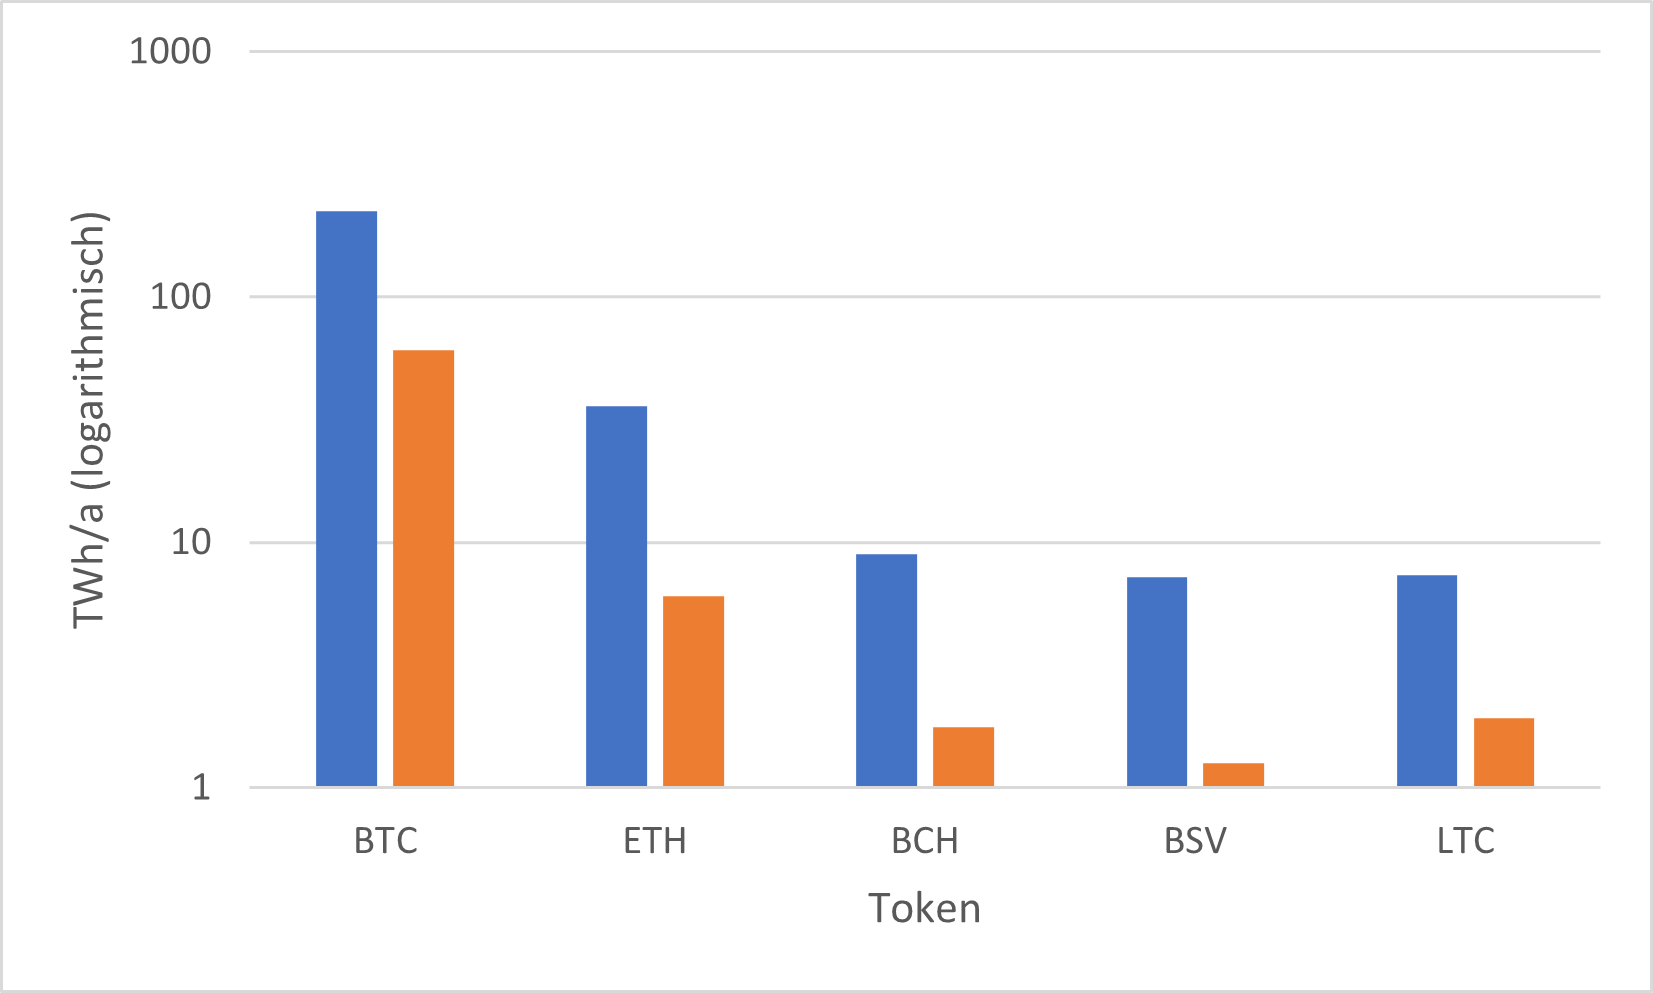
\includegraphics[width=.75\textwidth]{quellen/pow_2020.png}
    \caption{Stromverbrauch von PoW-Netzwerken 2020}
\end{figure}
\FloatBarrier
\clearpage
\noindent Als Vergleichsgröße zur Beliebtheit der Kryptowährungen eignet sich deren Marktkapitalisierung. Diese wird aus dem aktuellen Preis und der Umlaufmenge gebildet\citebib{cmcPoW}{}{vgl. }. Die Marktkapitalisierung der einzelnen Tokens im Jahre 2020 zeigt folgende Verteilung\citebib{sedlmeir}{S.602}{vgl. }:
\FloatBarrier
\begin{figure}[ht!]
    \centering
    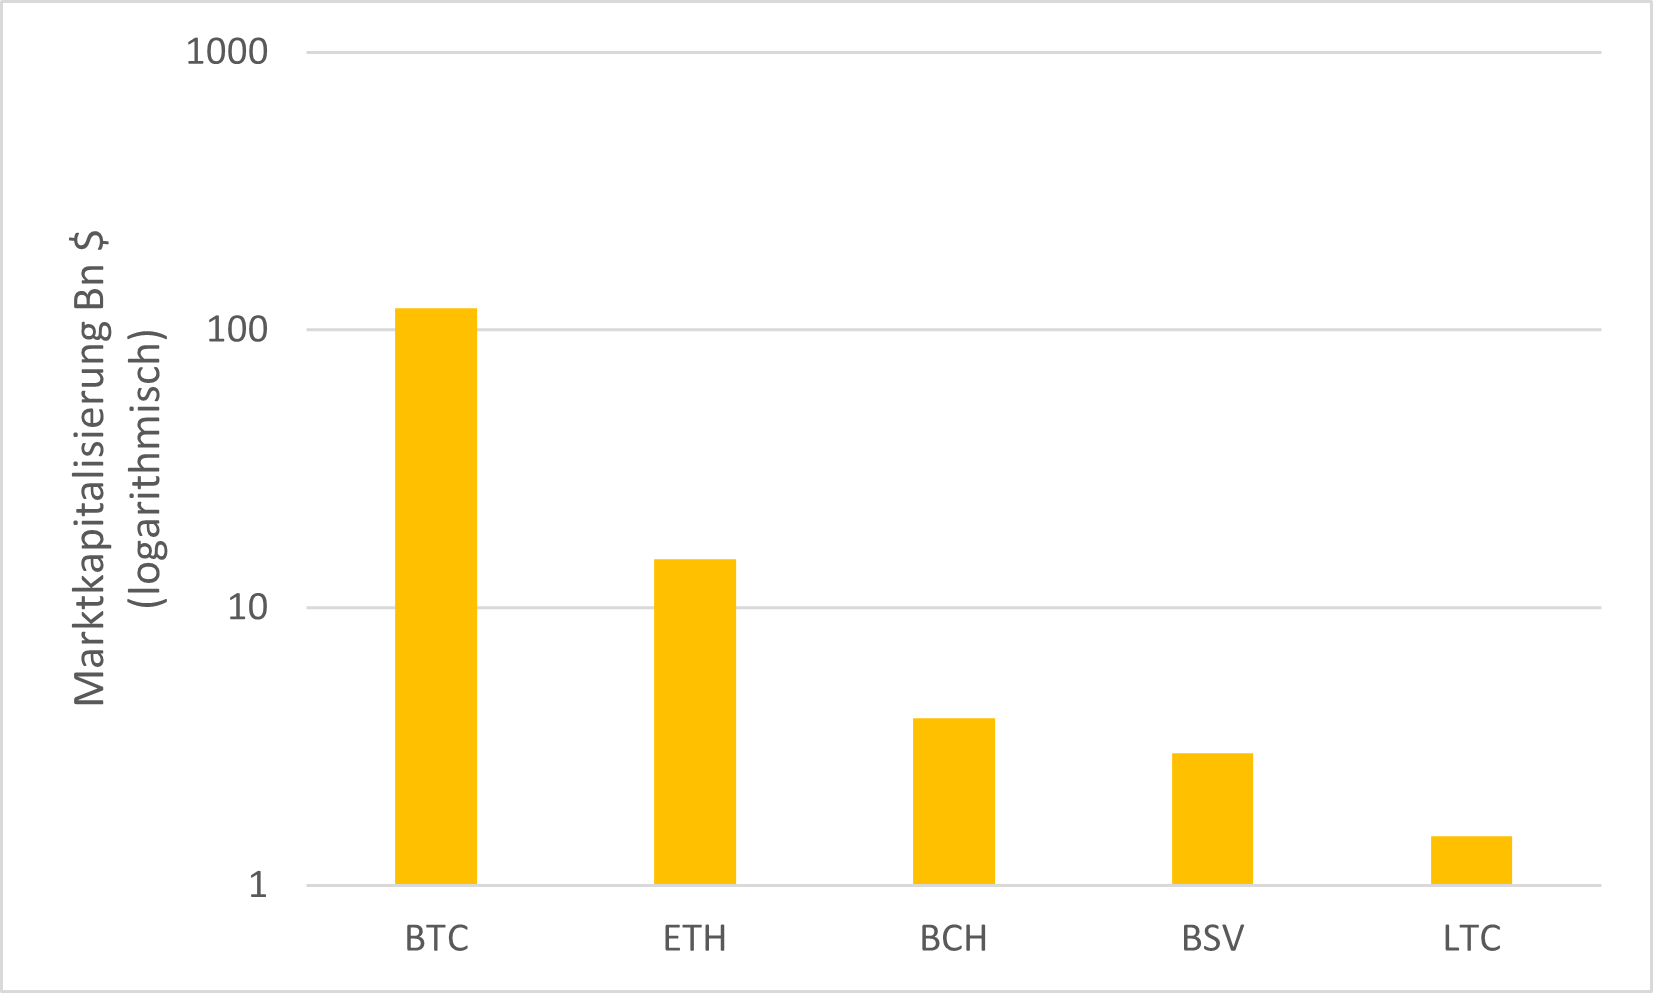
\includegraphics[width=.75\textwidth]{quellen/pow_mkp_2020.png}
    \caption{Marktanteil von PoW-Netzwerken 2020}
\end{figure}
\FloatBarrier

\subsection{Die Bedeutung des Energieverbrauchs}
Aus den von Johannes Sedlmeir und seinen Kollegen ermittelten Zahlen lässt sich schließen, dass die Verbreitung und der Preis eines Coins in Korellation zur verbrauchten Energie stehen\citebib{sedlmeir}{S.601f.}{vgl. }. Dieser Zusammenhang entspricht dem Grundprinzip des \textit{homo oeconomicus}. Bei der Untergrenze des Verbrauchs spiegelt dies sich in der Anzahl der pro Stunde gefundenen Blöcke wider, da die Teilnehmer im Netzwerk bei rentableren Coins mehr Rechenaufwand investieren und folglich mehr Blöcke gefunden werden. Bei der Obergrenze ist die Entlohnung des Miners direkt vom Preis der Coins abhängig.\\
Wenn die Stromkosten für die Erstellung eines neuen Blockes also höher als die Belohnung sind, ist zu erwarten, dass Miner das Netzwerk verlassen\citebib{beincrypto}{}{vgl. }. Ein weiterer Grund könnte die mit dem Energieverbrauch verbundene CO\textsuperscript{2}-Belastung sein, da Nachhaltigkeit und Umweltschutz in der Öffentlichkeit immer mehr Aufmerksamkeit finden. Es gibt allerdings auch Argumentationen, dass der Energieverbrauch irrelevant sei, solange die Energie aus erneuerbaren Quellen stammt\citebib{joule}{S.1844}{vgl. }.

\section{Einordnung des Stromverbrauchs von PoS-Tokens}
Im Vergleich zu den PoW-Tokens ist der Stromverbrauch von PoS-Tokens aufgrund des reduzierten Rechenaufwandes und der wegfallenden Redundanz vernachlässigbar (vgl. Kapitel 1.x). Dadurch könnte ein höherer Marktanteil erhofft werden, da das Thema Nachhaltigkeit in der Gesellschaft immer mehr an Bedeutung gewinnt\citebib{joule}{S.1843}{vgl. } Aus diesem Grund steigen einige Krypto-Netzwerke auf PoS um, wie zum Beispiel Ethereum es aktuell tut. Laut deren Einschätzungen wird der Energieverbrauch des PoS-Ethereum-Netzwerkes lediglich im MWh- oder niedrigen GWh-Bereich liegen\citebib{ethere}{}{vgl. }. Diese globalen Energieverbräuche liegen zum Beispiel noch deutlich unter dem Energieverbrauch der Stadt Münster im Jahr 2015 und sind deshalb vernachlässigbar\citebib{muenster}{}{vgl. }.

\section{Vergleich der Marktanteile von PoW und PoS}
Um einen Eindruck zur Beliebtheit von PoW-basierten Kryptowährungen im Vergleich zu PoS-basierten zu erhalten, ist die Marktkapitalisierung eine aussagekräftige Kennzahl. Die am Markt erfolgreichsten Kryptowährungen für PoW und PoS  sind online auffindbar\citebib{coinmarket2}{}{vgl. }:
\FloatBarrier
\begin{figure}[ht!]
    \centering
    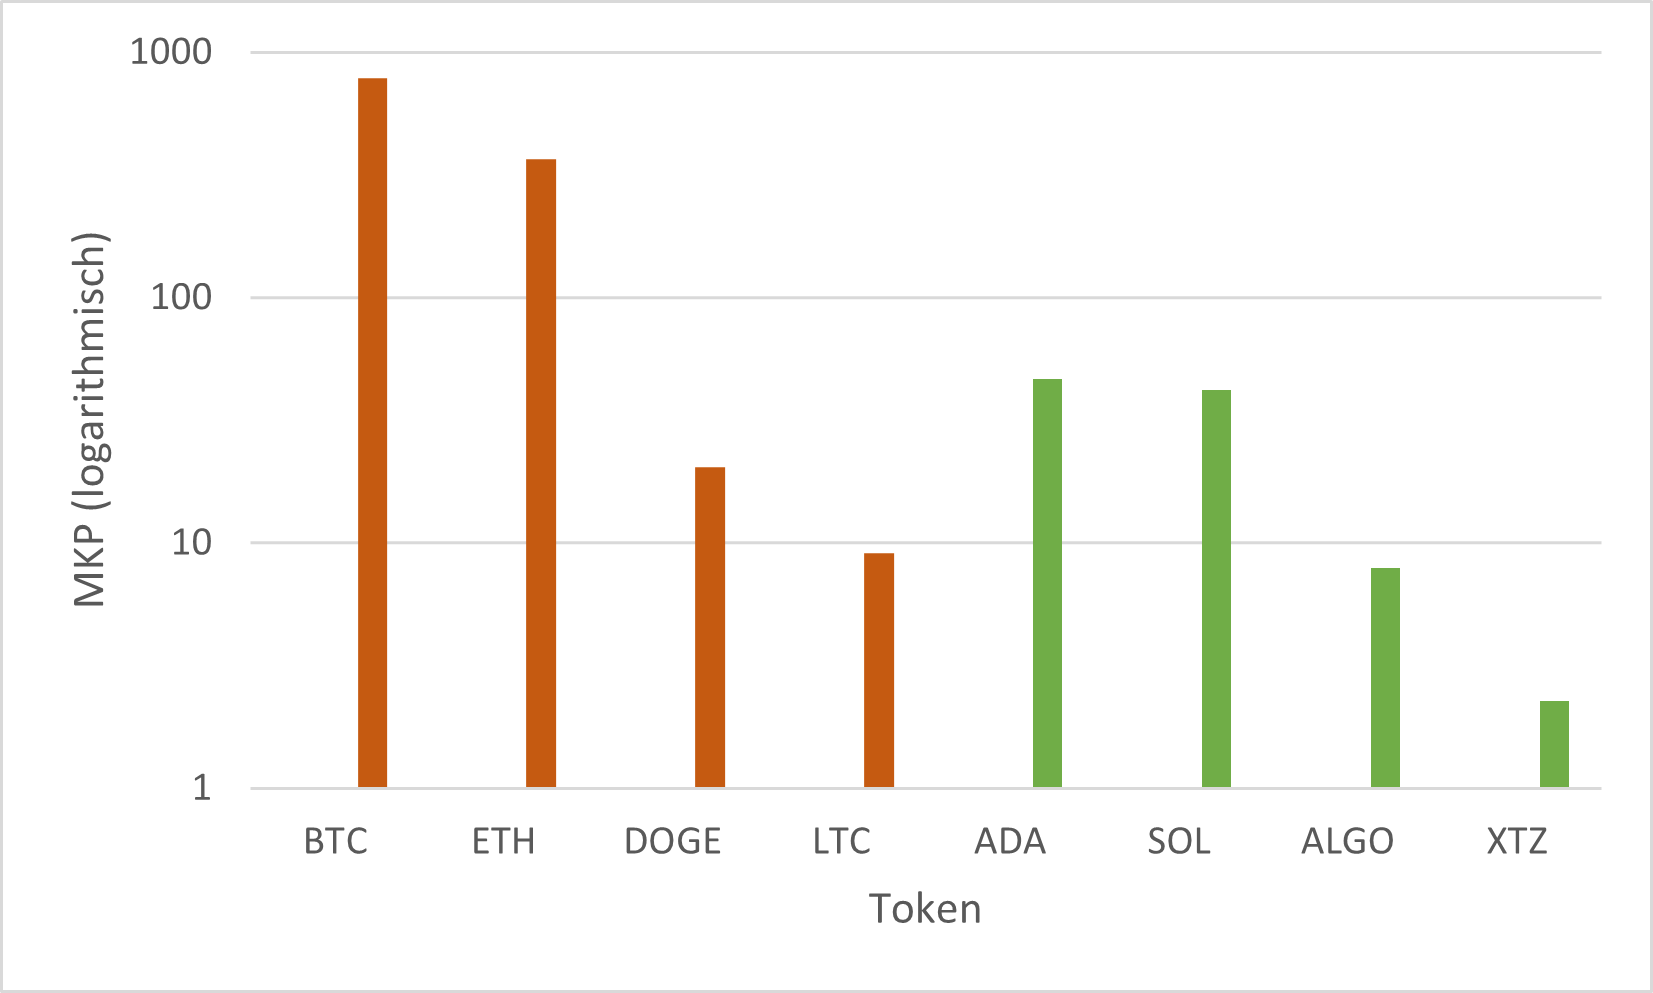
\includegraphics[width=.75\textwidth]{quellen/mkp_pow_pos.png}
    \caption{Vergleich Marktanteil von PoW- und PoS-Netzwerken 2022}
\end{figure}
\FloatBarrier
\noindent Wie zu erkennen ist, haben die beiden PoW-Tokens Bitcoin und Ethereum den größten Marktanteil. Allerdings verzeichnen PoS-Tokens, wie Cardano oder Solana über das letzte Jahr verteilt eine stetig anwachsende Marktkapitalisierung, während der Kurs der PoW-Tokens im Vergleich dazu stagniert.\citebib{coinmarket2}{}{vgl. }. Diese Entwicklung könnte darauf hindeuten, dass die energiesparenden PoS-Tokens in der Öffentlichkeit deutlich an Zuspruch gewinnen. Dies könnte ein weiterer ausschlaggebender Punkt dafür sein, dass Netzwerke wie Ethereum trotz ihrer hohen Marktkapitalisierung auf PoS umsteigen.

\section{Der gesamtheitliche Umwelteinfluss von Kryptowährungen}
Es bestehen verschiedene Möglichkeiten den negativen Einfluss von Kryptowährungen zu verringern, sowohl auf Seiten der Regierungen, als auch durch Unternehmen und die Wahl der Kryptowährung seitens Anwendern. Zwar ist Bitcoin und das verwendete Proof-of-Work Verfahren aktuell noch am bekanntesten, doch es bieten sich viele Alternativen, die nicht nur im Bezug auf Energieeffizienz, sondern auch in den Bereichen Sicherheit und Fairness Chancen bieten den Status quo zu verbessern. Trotzdem existieren gerade bezüglich alternativer Konsensverfahren noch Diskussionen im Bezug auf die Sicherheit, vor allem da viele Verfahren noch nicht in dem Maß getestet und erprobt sind wie das Proof-of-Work Verfahren. Solange diese Alternativen zum Proof-of-Work-Verfahren noch nicht ausgereift sind, ist ein ein Wechsel vom Bargeldsystem zu einer Kryptowährung aus ökologischer Sicht nicht zu empfehlen. Während eine Senkung der verbrauchten Energie also dringend gefordert wird, müssen erste Schritte seitens der Länder, Unternehmen und Einzelpersonen ergriffen werden, um einen Wechsel zu ermöglichen und durch Forschungsdaten die Folgen von alternativen Verfahren zu beurteilen.

\part{Methoden zum Vergleich des Umwelteinfluss von Kryptowährungen und dem klassischen Bargeldsystem}

\section{Life Cycle Assessment}
Das Life Cycle Assessment (LCA), im Deutschen auch Ökobilanz genannt, ist eine Methode, welche die Einflüsse der Produktion und Anwendung von Produkten auf die Umwelt aufzeigen soll. Die Methode wird in den ISO-Normen ISO 14040\citebib{iso2009}{}{vgl. } und ISO 14044\citebib{iso2006}{}{vgl. } beschrieben. Das LCA soll unter anderem dabei helfen, Verbesserungsmöglichkeiten für Produkte in Bezug auf ihre Umwelteigenschaften zu finden, Entscheidungsträgern in der Politik oder der Wirtschaft mit entsprechenden Informationen zu versorgen und die Auswahl von Indikatoren und Messverfahren für die Umwelteigenschaften zu vereinfachen. Außerdem kann die Ökobilanz zu Marketingzwecken von Unternehmen verwendet werden, um die Umwelteinflüsse ihrer Produkte aufzuzeigen\citebib{iso2009}{}{vgl. }.\\
Wie der englische Name „Life Cycle Assessment“ bereits vermuten lässt, wird bei dieser Methode der gesamte Lebensweg eines Produktes betrachtet. Dabei wird eine LCA-Studie in vier Phasen unterteilt\citebib{iso2009}{}{vgl. }:
\begin{enumerate}
    \item Festlegung des Ziels und des Untersuchungsrahmens
    \item Sachbilanz-Phase
    \item Wirkungsabschätzung
    \item Auswertung
\end{enumerate}
Da in den einzelnen Phasen die Erkenntnisse der anderen Phasen verwendet werden, handelt es sich bei der Ökobilanz um eine iterative Methode. Dieser Zusammenhang zwischen den Phasen wird in der folgenden Abbildung deutlich.
\FloatBarrier
\begin{figure}[ht!]
    \centering
    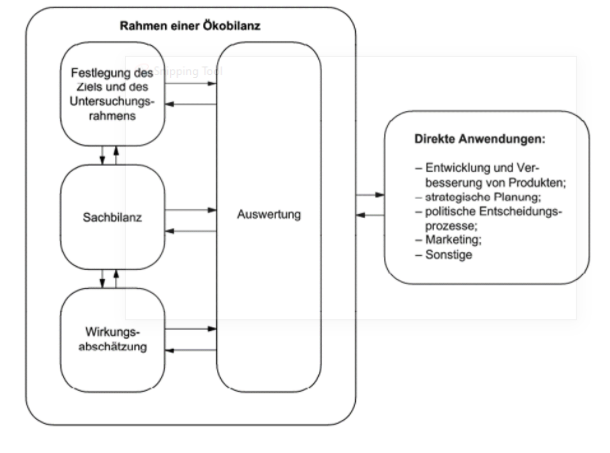
\includegraphics[width=.75\textwidth]{quellen/oekobilanz.png}
    \caption[Phasen einer Ökobilanz]{Phasen einer Ökobilanz (\textit{DIN EN ISO 14040:2009-11}, S.16)}
\end{figure}
\FloatBarrier

\subsection{Festlegung des Ziels und des Untersuchungsrahmens}
In der ersten Phase des Life Cycle Assessments werden zunächst das Ziel und der Untersuchungsrahmen definiert. Das Ziel beinhaltet die beabsichtigte Anwendung und die Gründe für die Durchführung der Studie. Weiterhin gibt es an, welche Zielgruppe angesprochen werden soll und ob die Ergebnisse zur Veröffentlichung bestimmt sind. Um sicherzustellen, dass der Detaillierungsgrad der Studie für das Ziel ausreichend ist, muss der Untersuchungsrahmen hinreichend definiert sein. Dieser beinhaltet das zu untersuchende Produktsystem und seine Funktion, die Systemgrenze, die Anforderungen an die Datenqualität und weitere Aspekte. Durch die iterative Herangehensweise kann der Untersuchungsrahmen sich im Laufe der Studie verändern. Dies kann zum Beispiel durch Erkenntnisse in der Sachbilanz erforderlich werden \citebib{iso2009}{, S.22ff.}{vgl. }.


\subsection{Sachbilanz}
Zu der Sachbilanz gehören Datenerhebungen und Berechnungsverfahren, welche verwendet werden, um Input und Output eines Produktsystems zu quantifizieren. Bei der Datenerhebung werden die Daten in Hauptgruppen unterteilt. Diese Hauptgruppen können zum Beispiel Energie-Inputs, Rohstoff-Inputs, Abfall, Emissionen oder weitere umfassen. Nach der Datenerhebung werden Berechnungsverfahren verwendet, um die gesammelten Daten zu validieren und den Prozessmodulen oder funktionellen Einheiten zuzuordnen\citebib{iso2009}{, S.25ff.}{vgl. }.

\subsection{Wirkungsabschätzung}
Die Ergebnisse der Sachbilanz werden in der nächsten Phase, der Wirkungsabschätzung, verwendet, um die potenziellen Umweltwirkungen des Produktes zu beurteilen. Hierbei werden Kategorien und Indikatoren verwendet, um die Auswirkungen zu erkennen. Die Wirkungsabschätzung kann auch verwendet werden, um festzustellen, ob das Ziel der Studie erreicht wurde\citebib{iso2009}{, S.25ff.}{vgl. }.\\
Bei der Auswahl einer Wirkungsabschätzungsmethode kann zwischen zwei grundlegenden Ansätzen unterschieden werden. Der erste ist der sogenannte „Midpoint“-Ansatz, welcher Problem-orientiert ist. Bei dieser Methode werden die Wirkungsindikatoren nah an der Ursache definiert. Das Gegenstück zu diesem Ansatz ist der „Endpoint“-Ansatz. Die Wirkungsindikatoren bei diesem Ansatz beschreiben meist den entstehenden Schaden, weshalb ihre Relevanz für die Umwelt höher ist als beim „Midpoint“-Ansatz. Eine Methode, welche beide Ansätze verbindet, ist die ReCiPe-Methode\citebib{bruijn}{S.530}{vgl. }.

\subsection{ReCiPe}
Die ReCiPe-Methode ist eine Methode zur Umsetzung einer Wirkungsabschätzung. Sie verwendet 18 Wirkungskategorien auf der „Midpoint-Ebene“ und fasst diese zu 3 Kategorien auf der „Endpoint-Ebene“ zusammen. Die drei Endpoint-Kategorien sind menschliche Gesundheit, Vielfalt der Ökosysteme und Ressourcenverfügbarkeit. Aus diesen drei Endpunkten wird dann ein einzelner Indikator berechnet, welcher in sogenannten „Ecopoints“ (Pt) ausgedrückt wird. Mit diesem Indikator lassen sich verschiedene Produkte bezüglich ihrer Umweltwirkung vergleichen\citebib{goedkoop}{S.2f.}{vgl. }.
Die drei Endpunkte sind als schützenswerte Bereiche deklariert, und haben jeweils einen Indikator, um die Auswirkungen auf diese Bereiche zu messen.\\
Die erste Kategorie, menschliche Gesundheit, verwendet als Indikator die sogenannten disability-adjusted life years (DALY). Auf Deutsch könnte dieser Indikator als verlorene gesunde Lebensjahre übersetzt werden. Beim DALY-Konzept werden die verlorenen Lebensjahre durch Tod oder Behinderung summiert und als Kennzahl dargestellt\citebib{goedkoop}{S.7f.}{vgl. }.\\
Die Vielfalt der Ökosysteme wird durch den Verlust von Spezies in einem Jahr bemessen. Ökosysteme sind sehr komplex und es ist extrem schwierig diese anhand einer Kennzahl abzubilden. Dennoch wird bei der ReCiPe-Methode die Annahme getroffen, dass sich die Qualität eines Ökosystems durch die Vielfalt der Spezies ausreichend bemessen lässt\citebib{goedkoop}{S.8ff.}{vgl. }.\\
Ein großes Problem der Zukunft wird vermutlich sein, dass der Menschheit die Ressourcen ausgehen werden. Dieses Problem wird in der dritten Kategorie, der Ressourcenverfügbarkeit, festgehalten. Hierbei wird die durch die Verwendung von Ressourcen entstehende Grenzkostensteigerung für die zukünftige Extraktion von Ressourcen als Indikator herangezogen. Da eine Erhöhung der Kosten für Öl einen deutlich höheren Einfluss auf die Gesellschaft hat, als die Erhöhung der Kosten für zum Beispiel Quecksilber, werden die Grenzkostensteigerungen für verschiedene Ressourcen unterschiedlich gewichtet. So wird die Schwere der Auswirkungen einer Kostenerhöhung mit einbezogen. Der Indikator wird in Dollar angegeben\citebib{goedkoop}{S.10ff.}{vgl. }.
\FloatBarrier
\begin{figure}[ht!]
    \centering
    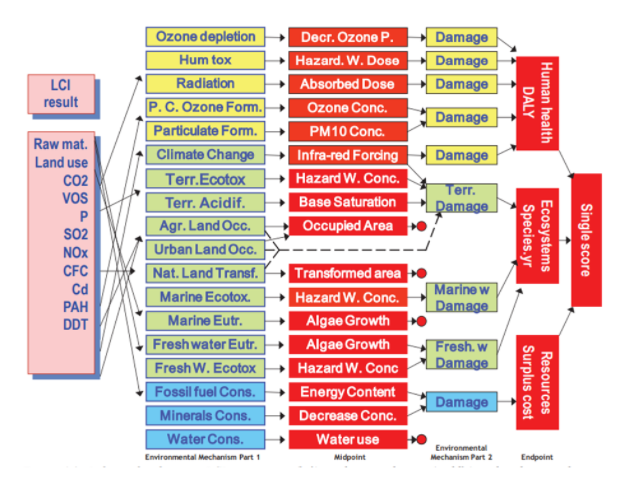
\includegraphics[width=.75\textwidth]{quellen/recipe.png}
    \caption[Zusammenhang der verschiedenen Indikatoren der ReCiPe-Methode]{Zusammenhang der verschiedenen Indikatoren der ReCiPe-Methode (\textit{Geodkoop et al}, S.3)}
\end{figure}
\FloatBarrier

\subsection{Auswertung}
In der letzten Phase, der Auswertung, werden die Erkenntnisse aus der Sachbilanz und der Wirkungsabschätzung verwendet, um Ergebnisse zu erhalten, die mit dem Ziel und dem Untersuchungsrahmen übereinstimmen und eine Schlussfolgerung ermöglichen. Mit den Ergebnissen der Auswertung können dann zum Beispiel Empfehlungen ausgesprochen werden. Die Auswertung sollte außerdem eine leicht verständliche und vollständige Darstellung der Ergebnisse beinhalten\citebib{iso2009}{, S.31f.}{vgl. }.

\section{Beispielhafte Umsetzung eines Life Cycle Assessments}
Das Life Cycle Assessment ist vor allem dazu geeignet verschiedene Produkte bezüglich ihrer Umweltwirkung zu vergleichen. Durch die Verwendung der ReCiPe-Methode können die Ergebnisse am Ende anhand einer Kennzahl beziffert und verglichen werden. Eine mögliche Umsetzung eines solchen Assessments soll im Folgenden beispielhaft anhand des klassischen Bargeldsystems und anhand einer Kryptowährung aufgezeigt werden.
\subsection{Bargeldsystem}
Die Niederländische Bank hat 2018 eine Studie über die Auswirkungen des niederländischen Bargeldsystems auf die Umwelt und den Klimawandel aus 2015 veröffentlicht. In dieser Studie wird ein Life Cycle Assessment in Kombination mit der ReCiPe 2008 (H) Methode durchgeführt. Das Ziel der Studie ist es, einen quantitativen Einblick in die Auswirkungen des niederländischen Bargeldsystems auf die Umwelt zu erhalten und die Ergebnisse der Studie zu veröffentlichen. Für den Untersuchungsrahmen wurden zwei funktionale Einheiten bestimmt. Die erste Einheit ist das gesamte niederländische Bargeldsystem mit allen Transaktionen aus 2015. Die zweite funktionale Einheit ist eine durchschnittliche Bargeldzahlung in den Niederlanden in 2015, welche hinzugefügt wurde, um am Ende eine einzelne Bargeldzahlung mit einer einzelnen Debitkartenzahlung zu vergleichen\citebib{nlbank}{S.4}{vgl. }.\\
Für die Sachbilanz wurde das Bargeldsystem in fünf Subsysteme unterteilt. Die Produktion von Banknoten, die Produktion von Münzen, die operative Phase, die End-of-Life-Phase der Banknoten und die End-of-Life-Phase der Münzen. Diese Subsysteme wurden in verschiedene Prozesse unterteilt, welche dann bei der Datenerhebung betrachtet wurden, um die Umweltwirkung der Subsysteme zu berechnen. Die genaue Unterteilung ist in der nachfolgenden Grafik zu erkennen\citebib{nlbank}{S.5ff.}{vgl. }.
\FloatBarrier
\begin{figure}[ht!]
    \centering
    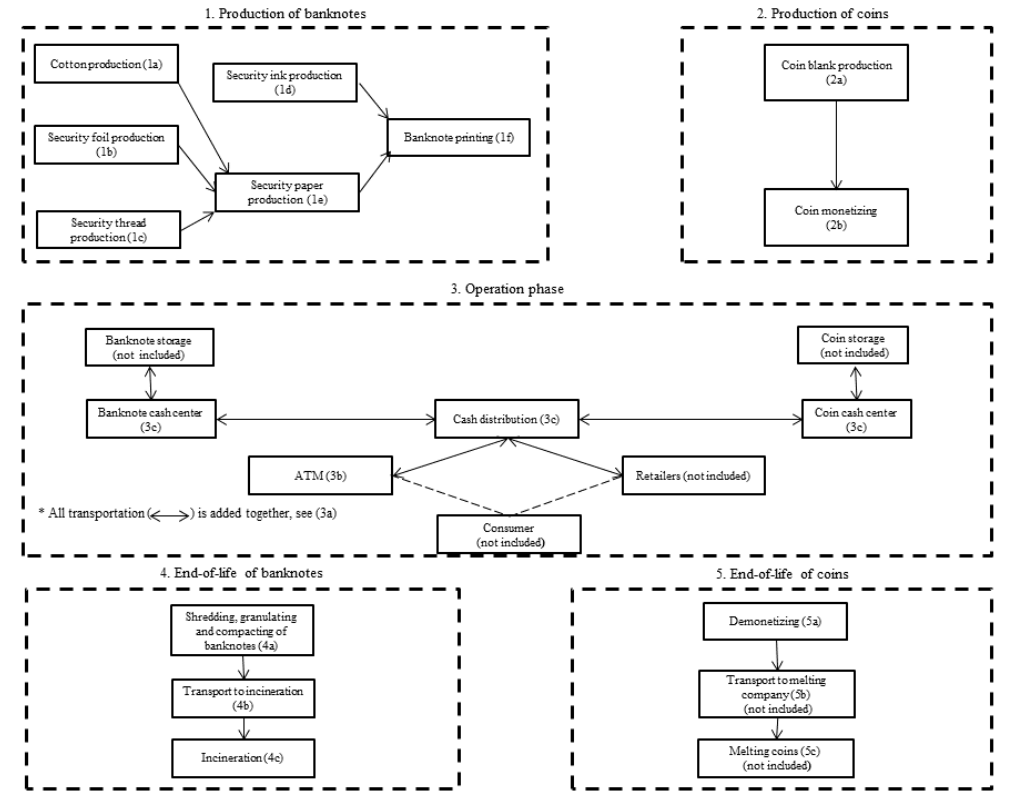
\includegraphics[width=\textwidth]{quellen/bgsys.png}
    \caption[Der Lebenszyklus des Bargeldsystems in fünf Subsystemen]{Der Lebenszyklus des Bargeldsystems in fünf Subsystemen (\textit{Hanegraaf et al.}, S.5)}
\end{figure}
\FloatBarrier
\noindent Für die Wirkungsabschätzung wurde die ReCiPe (H) Methode verwendet, um die Umweltwirkung in Ecopoints zu berechnen. Dabei kam die Studie auf ein Ergebnis von 2,35 MPt (Millionen Ecopoints) für das gesamte niederländische Bargeldsystem. Der größte Anteil der Ecopoints ergab sich aus der operativen Phase mit 1,49 MPt. Danach kam die Produktion der Münzen mit 0,75 MPt und dann die Produktion der Banknoten mit 0,12 MPt. Die beiden End-of-Life-Phasen hatten einen insignifikanten Einfluss auf die Umwelt. Eine einzelne Bargeldzahlung belief sich auf 631 \begin{math}\mu Pt\end{math}\citebib{nlbank}{S.15}{vgl. }.\\
In der Auswertung wurden unter anderem verschiedene Szenarien diskutiert, welche Maßnahmen getroffen werden könnten, um die Auswirkungen auf die Umwelt zu reduzieren und wie sich diese Maßnahmen auf die Ecopoints niederschlagen würden\citebib{nlbank}{S.19ff.}{vgl. }.
\subsection{Kryptowährungen}
Neben der Studie der Niederländischen Bank gibt es ein veröffentlichtes Life Cycle Assessment, welches die Umweltauswirkungen des gesamten Euro-Bargeld-Systems mit dem Bitcoin-System vergleicht. Die erste Ökobilanz berechnete Umweltauswirkungen für das gesamte Euro-Bargeld-System in 2020 in Höhe von 59,98 MPt\citebib{pollani}{S.64}{vgl. }.\\
Das Ziel des zweiten Life Cycle Assessments ist es, eine Einschätzung über die Umweltauswirkungen des Bitcoin-Systems zu erhalten. Dabei wurden wie bei der Ökobilanz des Bargeldsystems zwei funktionale Einheiten definiert. Die berechneten Terahashes für alle erschaffenen Bitcoins in 2020 und die berechneten Terahashes für einen erschaffenen Bitcoin in 2020. Weiterhin wurde die Eingrenzung getroffen, dass nur die Umweltwirkungen betrachtet werden, die durch den Energiebedarf beim Mining verursacht werden \citebib{pollani}{S.67ff.}{vgl. }.\\
Für die Sachbilanz wurde die Anzahl aller geschöpften Bitcoins in 2020 berechnet. Diese Anzahl belief sich auf 445.500 neue Bitcoins. Die für Bitcoin-Mining verwendete Hardware hat in den letzten Jahren vier Generationen durchlaufen. Zu Beginn wurden einfache Prozessoren (CPU) von PCs verwendet. Danach wechselte man zu Grafikkarten (GPU), dann zu Field Programmable Gate Arrays (FPGA) und schließlich zu Application-Specific Integrated Circuits (ASIC). Bei ASICs handelt es sich um Hardware-Chips, welche darauf spezialisiert sind, Hash-Berechnungen möglichst effizient durchzuführen\citebib{pollani}{S.73ff.}{vgl. }.\\
Um den durchschnittlichen Energiebedarf von ASICs beim Bitcoin-Mining zu bestimmen, wurden die Kennzahlen der am meist verbreitesten ASICs gewichtet und zusammengerechnet. Dabei kam man zu dem Ergebnis, dass ein ASIC durchschnittlich 0,0000202 kWh pro Terahash verbraucht. Weiterhin wurde die Anzahl der generierten Hashes berechnet. Diese lag bei 3.763.662.734.304.180 Th in 2020, was bedeutet, dass durchschnittlich 8.448.176.732 Th pro geschöpften Bitcoin berechnet wurden. Abschließend wurde der beim Bitcoin-Mining verwendete Energiemix herangezogen, um zu berechnen, wie viel Strom ein durchschnittlicher ASIC aus Wasserkraft, geothermischer Stromerzeugung und Kohlekraftwerken bezieht\citebib{pollani}{S.73ff.}{vgl. }.
\FloatBarrier
\begin{figure}[ht!]
    \centering
    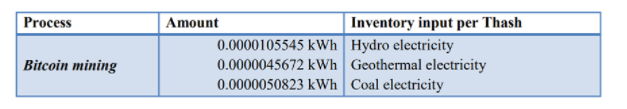
\includegraphics[width=.75\textwidth]{quellen/btc_mining_numbers.png}
    \caption[Energiemix für durchschnittliche ASIC]{Energiemix für durchschnittliche ASIC (\textit{Pollani Federica}, S.75)}
\end{figure}
\FloatBarrier
\noindent Diese Daten wurden dann in der Wirkungsabschätzung verwendet, um mithilfe der ReCiPe (H) Methode die Ecopoints für Bitcoins zu berechnen. Die berechneten Ecopoints für das gesamte Bitcoin-System in 2020 betrugen 1.358,41 MPt. Der gesamte Energiebedarf betrug 76,03 TWh \citebib{pollani}{S.76}{vgl. }.\\
Damit hat das Bitcoin-System deutlich größere Auswirkungen auf die Umwelt, als das gesamte Euro-Bargeld-System (59,98 MPt). Dennoch muss dieser Vergleich mit Vorsicht genossen werden. Die Studie hat lediglich ein Bargeldsystem mit nur einem Kryptowährungssystem verglichen. Auch ist zu beachten, dass der Euro hauptsächlich in Europa und der Bitcoin global verwendet und hergestellt wird. Nichtsdestotrotz lässt sich sagen, dass sich ein Wechsel von einem Bargeldsystem auf ein Kryptowährungssystem mit den aktuell verwendeten Berechnungsverfahren negativ auf die Umwelt auswirken würde.

\part{Verbesserung der Auswirkungen von Crypto-Mining auf die Umwelt}
\section{Ursachen und Ansätze}
\input{chapters/Verbesserungen/Ursachen.tex}

\section{Grüner Strom}
Eine Möglichkeit, um negative Auswirkungen auf die Umwelt durch Kryptowährungen zu verringern, ohne dass der generelle Stromverbrauch dabei gesenkt werden muss, ist das Beziehen des Stroms aus erneuerbaren Quellen und somit die Verwendung von „grünem Strom“.\\
Kryptowährungen bedienen sich meist Blockchain-Verfahren und nutzen die Vorteile des damit erbauten dezentralen Systems. Gerade diese Dezentralisierung erschwert allerdings auch die Ermittlung von aktuellen Werten zu verwendeten Stromquellen. Für eine offene, nicht zugangsbeschränkte Proof-of-Work-Blockchain ist bereits der Stromverbrauch nur schwer bestimmbar, da „[…] man in der Regel weder die beim Mining eingesetzte Rechenleistung noch die entsprechende Hardware für jeden Teilnehmer bestimmen kann.“\citebib{infoSpektrum}{S.394}{}. Der Standort, sowie weitere Faktoren wie der technische Stand der Ausrüstung und das vorherrschende Klima, beeinflussen wiederum den Energieverbrauch und die CO2-Emissionen. Diese Faktoren in Kombination mit fehlenden Daten über Miner und deren Ausrüstung führen zu einer Unsicherheit in den ermittelten Werten zum Stromverbrauch und Umwelteinfluss, die sich in auseinandergehenden Kennzahlen niederschlägt. Beispielsweise werden laut einer Studie von Cambridge bereits durchschnittlich 39\% des Proof-of-Work Mining mit erneuerbaren Energien durchgeführt\citebib{blandin}{S.26}{vgl. }. Andere Studien, wie die der CoinShares Research, gehen sogar von einem Prozentanteil von 74\% beim Bitcoin-Mining aus\citebib{bendiksen}{}{vgl. }.\\
Neben den genannten Faktoren spielt auch die ständige Weiterentwicklung und Veränderung der Hauptstandorte von Mining-Farmen und Minern eine Rolle. Ein Beispiel dafür ist das 2021 erlassene Verbot der chinesischen Regierung gegen Bitcoin, durch das China von einem Anteil von geschätzten 46,04\% an der Netzwerk-Hash-Rate im April 2021 auf mittlerweile 0\% gefallen ist. Andere Länder, wie beispielsweise Amerika, profitierten anschließend von einem Zuwachs an Minern\citebib{btcDist}{}{vgl. }. Durch eine solche Verschiebung der Anteile bzw. Standorte ändert sich ebenfalls die Zusammensetzung der für das Mining verwendeten Energiequellen, die ihrerseits abhängig von den Bezugsquellen des jeweiligen Landes sind.\\
Im Allgemeinen sind die Aussichten auf eine Senkung der CO2-Emissionen durch „grünen Strom“ durchaus positiv einzuschätzen, da eine Verwendung von erneuerbaren Energien sich für die Miner als wirtschaftlich lohnend zeigt. Insbesondere bei dem Konsensmechanismus des Proof-of-Work, bei dem die Wahrscheinlichkeit den nächsten Block schreiben zu dürfen mit der Rechenleistung steigt, muss der Ertrag durch durchschnittlich gewonnene Einheiten der Kryptowährung größer sein als der Aufwand durch den verwendeten Strom und gegebenenfalls auch angeschaffte Hardware. Je höher die Differenz zwischen Ertrag und Aufwand dabei ist, desto höher fällt auch der Gewinn aus, sodass ein möglichst günstiger Strompreis essentiell für die Höhe des Gewinns ist. Strom aus erneuerbaren Energien bietet sich hierbei an, da dieser oftmals günstiger und somit wirtschaftlich vorteilhafter für die Miner ist\citebib{irena}{}{vgl. }.\\
Zu beachten ist allerdings die Abhängigkeit vom Standort und in die dortige Verfügbarkeit von Strom aus erneuerbaren Energien. Sollten Miner von einem Land aus agieren, dass sich beispielsweise hauptsächlich auf Strom aus Kohlekraftwerken stützt, müssten sie sich dem für sie zugänglichem Strom bedienen, oder wären gezwungen ihren Standort zu wechseln. Diese Zuständigkeit der Länder bietet sowohl Vor- als auch Nachteile. Zwar gewinnen diese an Entscheidungsmacht und können Maßnahmen unabhängig von den Systemen der Kryptowährungen vornehmen, allerdings gehen diese Maßnahmen nicht die Ursache des Problems – allen voran der Konsensmechanismus – an, sondern dämmen lediglich die Schäden ein. Zudem könnte eine Entwicklung, durch die Strom aus umweltschädlichen oder nicht erneuerbaren Energien günstiger wird, dazu führen, dass Miner dem Prinzip der Gewinnmaximierung folgend diese Variante wählen.


\section{Diskussion alternativer Konsensmechanismen}
%\subsection{Konsensmechanismen}
Da viele der Kryptowährungen die Blockchain-Technologie nutzen und in einem solchen dezentralen Netzwerk eine Notwendigkeit besteht sich auf bestimmte Status oder Datenwerte zu einigen, werden Konsensverfahren eingesetzt. Eines der bekanntesten Verfahren, das in Kapital 2.4.2 bereits erläutert wurde ist dabei das Proof-of-Work Verfahren. Wie die meisten Konsensverfahren fordert auch Proof-of-Work eine Art von Einsatz, um an der Auswahl zum Schreiben des nächsten Blocks teilzunehmen. Proof-of-Work nutzt hierbei die Rechenleistung als seine Art von Einsatz, was in der Kombination mit der Konkurrenz um jeden Block zu dem hohen Energieverbrauch führt. Allerdings gibt es weitere, alternative Konsensverfahren, die mit einem anderen Einsatz arbeiten und somit den Energieverbrauch und auch die Verschwendung von Energie senken.\\
Die Kryptowährung Ether, die bisher ebenso wie Bitcoin den Proof-of-Work Mechanismus verwendet hat, befindet sich beispielsweise aktuell in einer Umstellung auf den Proof-of-Stake-Mechanismus. Auch andere Mechanismen könnten eine umweltschonende Alternative zu dem Status quo bieten. Einige solcher alternativen Mechanismen sollen im Folgenden genauer betrachtet werden.

\subsection{Proof-of-Stake}
Das Proof-of-Stake Verfahren ist einer der bekanntesten Konsensmechanismen neben dem Proof-of-Work und agiert über eine zufällige, aber gewichtete Auswahl des Validatoren. Das für die Gewichtung betrachtete Kriterium ist dabei der eingesetzte Stake, eine bestimmte Menge von Kryptowährung, die als Einsatz genutzt wird. Abhängig von der Höhe des Stakes wird so ein Validator bestimmt, der den nächsten Block schreiben darf und die dafür angesetzte Transaktionsgebühr bekommt\citebib{hazari}{}{vgl. }.\\
Durch den Wegfall der Konkurrenz ist der Energieverbrauch im Vergleich zum Proof-of-Work Verfahren um einiges geringer und auch die Notwendigkeit zu spezieller Ausrüstung, um an der Auswahl teilzunehmen, entfällt.\\
Allerdings verschafft das Proof-of-Stake Verfahren Personen, die bereits viele Einheiten der Kryptowährung besitzen einen Vorteil, sodass „reiche“ Personen eine höhere Chance haben ausgewählt zu werden. Um dem entgegenzuwirken können weitere Faktoren zur Auswahl mit einbezogen werden, beispielsweise die Dauer, über welche eine Person bereits im Besitz seiner Menge an Kryptowährung ist oder wie lange er seinen Stake bereits gesetzt hat\citebib{hazari}{}{vgl. }.\\
Ein weiterer zu berücksichtigender Faktor ist die Sicherheit, die das Proof-of-Stake Verfahren bietet. Validiert jemand einen manipulierten oder gefälschten Block und wird dabei erwischt, wird demjenigen ein Teil bzw. sein gesamter Stake entzogen, sodass Teilnehmer zur Aufrichtigkeit angehalten werden. Abgesehen von diesem Aspekt gibt es jedoch Bedenken bzgl. der konzeptionellen und technischen Sicherheit des Proof-of-Stake-Verfahrens. Im Vergleich zum Proof-of-Work-Verfahren ist dieses anfälliger für bestimmte Angriffe und bringt somit ein höheres Risiko mit sich\citebib{nair}{}{vgl. }. Ausgenommen hiervon ist allerdings der sogenannte 51\%-Angriff. Durch einen solchen Angriff schafften es Hacker bei Bitcoin Gold Coins in einem Wert von bis zu 18 Millionen Dollar zu erbeuten, indem sie Kryptowährung doppelt ausgaben. Ein solcher Angriff würde in einem System mit dem Proof-of-Stake Verfahren erheblich erschwert, da zur Durchführung 51\% der Coins nötig wären und ein Angreifer Gefahr stünde, diese durch den Angriff zu verlieren\citebib{suhyeon}{}{vgl. }. Jedoch gibt es auch hier bereits Theorien, laut denen ein solcher Angriff auf ein Proof-of-Stake System nicht nur durchführbar, sondern auch potenziell lohnend für den Angreifer sein und das gesamte Proof-of-Stake Kryptowährungssystem eventuell sogar zerstören könnte (vgl. ebd.)\citebib{houy}{}{vgl. }.

\subsection{Proof-of-Importance}
Das Proof-of-Importance Verfahren ähnelt dem Proof-of-Stake Verfahren und ist gleichzeitig ein Ansatz, um dem in letzterem festgestellten Problem der Bevorzugung von reichen Personen entgegenzuwirken. Hierzu werden neben dem Vermögen auch die Haltedauer und die Aktivität der Person zu einem sogenannten Importance-Score verrechnet. Auf diese Weise sollen Personen gefunden werden, die besonders wichtig für das System sind und somit ein hohes Interesse an dem Fortbestehen und der Korrektheit des Systems haben. Teilnehmer, die sehr aktiv sind, also viele Transaktionen durchführen, haben eine höhere Chance als Validator für den nächsten Block ausgewählt zu werden\citebib{hazari}{}{vgl. }.\\
Durch die Auswahl eines Validators entfallen auch hier die Aufwände der Konkurrenz und die Notwendigkeit für spezielle technische Ausrüstungen, um an der Auswahl teilnehmen zu können. Allerdings führt die Verwendung des Proof-of-Importance Verfahrens auch dazu, dass es für neue Teilnehmer zunächst schwierig ist als Validator ausgewählt zu werden und auch eine lange Abwesenheit bzw. Inaktivität wirkt sich negativ auf die Chance Validator zu werden aus.

\subsection{Proof-of-Space}
Der Proof-of-Space-Mechanismus, oder auch Proof-of-Capacity genannt, fordert als seine Art von Einsatz Festplattenspeicher. Ein einzelner “Proof-of-Space” bezeichnet dabei Daten, die belegen, dass ein Anwender eine bestimmte Menge an Speicherplatz reserviert hat\citebib{he}{}{vgl. }. Was folgt ist ein Vorgang der im Rahmen des Burstcoin Netzwerks auch als Plotting bezeichnet wird. Berechnungen werden einmalig durchgeführt und die Ergebnisse anschließend gespeichert, sodass sie später beim Mining schlichtweg ausgelesen werden können. Die Wahrscheinlichkeit für die Validierung ausgewählt zu werden steigt dabei proportional mit dem bereitgestellten Speicher. Auf diese Weise wird der Energieverbrauch im Vergleich zum Proof-of-Work Verfahren gesenkt, allerdings könnte der Einsatz dazu führen, dass die Konkurrenz um Rechenleistung sich zu einer Konkurrenz um Speicherplatz entwickelt\citebib{hazari}{}{vgl. }.

\subsection{Proof-of-Burn}
Seinem Namen entsprechend fordert der Proof-of-Burn Konsensmechanismus von Minern das „Verbrennen“ von Kryptowährung als seinen Einsatz. Das sogenannte „Verbrennen“ beschreibt dabei den Transfer von Coins zu einer Adresse, auf die kein Zugriff besteht, auch nicht seitens des Senders\citebib{verma}{}{vgl. }. Dorthin verschickte Coins können also auch nicht mehr eingesetzt werden und werden dem System gewissermaßen entzogen bzw. „zerstört“.\\
Beim Proof-of-Burn verbrennen Miner auf diese Weise einen Teil ihrer Coins, meist die einer anderen Kryptowährung, um sich für die Validierung als vertrauenswürdig zu erweisen. Je höher dabei die Menge der über die Zeit zerstörten Coins ist desto höher ist auch die Chance für die Validierung des nächsten Blocks ausgewählt zu werden\citebib{he}{}{vgl. }. Um den Verlust von Coins langfristig auszugleichen, werden dabei oftmals Belohnungen für jeden neuen Block ausgegeben.
Ein Vorteil dieses Konsensmechanismus ist, dass er sich nicht auf den Einsatz von Rechenleistung oder Hardware verlässt und somit abgesehen von den verbrannten Coins einen geringeren Aufwand verursacht\citebib{verma}{}{vgl. }. Die Sicherheit wird durch den hohen Einsatz in Form von Coins gewährleistet. Indem die Miner eine hohe Anfangsinvestition leisten, sollen sie so langfristig ehrlich und am System interessiert bleiben, um diese stetig zurückzuerlangen\citebib{hazari}{}{vgl. }.

\part{Fazit}
Es bestehen verschiedene Möglichkeiten den negativen Einfluss von Kryptowährungen zu verringern, sowohl auf Seiten der Regierungen, als auch durch Unternehmen und die Wahl der Kryptowährung seitens Anwendern. Zwar ist Bitcoin und das verwendete Proof-of-Work Verfahren aktuell noch am bekanntesten, doch es bieten sich viele Alternativen, die nicht nur im Bezug auf Energieeffizienz, sondern auch in den Bereichen Sicherheit und Fairness Chancen bieten den Status quo zu verbessern. Trotzdem existieren gerade bezüglich alternativer Konsensverfahren noch Diskussionen im Bezug auf die Sicherheit, vor allem da viele Verfahren noch nicht in dem Maß getestet und erprobt sind wie das Proof-of-Work Verfahren. Solange diese Alternativen zum Proof-of-Work-Verfahren noch nicht ausgereift sind, ist ein ein Wechsel vom Bargeldsystem zu einer Kryptowährung aus ökologischer Sicht nicht zu empfehlen. Während eine Senkung der verbrauchten Energie also dringend gefordert wird, müssen erste Schritte seitens der Länder, Unternehmen und Einzelpersonen ergriffen werden, um einen Wechsel zu ermöglichen und durch Forschungsdaten die Folgen von alternativen Verfahren zu beurteilen.

\clearpage
\frontmatter%Stil des Headers/Footers ändern
\renewcommand{\plaintitle}{Literaturverzeichnis}
\pagenumbering{Roman}
\setcounter{page}{5}
\addtocontents{toc}{\vspace{24pt}}
\addcontentsline{toc}{part}{Literaturverzeichnis}%Literatur-Verz. ins Inhaltsverzeichnis
\printMyBibliography

\end{document}